\chapter{Experimenteller Aufbau}
MYLAR FILTER MIT ALU


\noindent
Der Streuungseffekt der Proben ist sehr energieselektiv und ist deswegen nur im schmalen Bereich um der Resonanzenergie $h\nu_{\text{Fe, L3}}$ bzw. $h\nu_{\text{Gd, M5}}$ zu erwarten. Diese Energien sind jedoch nicht die Zielenergien der beiden \gls{rzp}. Aus diesem Grund muss der Strahl mit dem Fokuspunkt horizontal verschoben werden, damit die Resonanzenergie mittig an dem Detektor liegt und an die Probe projiziert werden kann. Mit der zunehmenden Entfernung von der Fokuspunkt nimmt die Effizienz und die Abbildungsschärfe, also der Energiebereich pro Längeeinheit entlang der Energieachse, der \gls{rzp} ab.


\noindent
Aus diesen Gründen kann der Photonenfluss von der bestimmten Photonenenergie, der schließlich auf den Detektor landet, nicht so einfach von der Abb. \ref{fig:pxs_spectrum} genommen werden, sondern muss experimentell bestimmt werden. Mit Einschub in den Abschnitt \ref{text:butterfly_counting} kann man sagen, dass die Gesamtzahl der Photonen in derselben Konfiguration der Abb. \ref{fig:butterfly_moench} pro ein Puls ca. 527 detektiert werden, wobei nur ca. ??? sich im Gd M5 markierten Bereich befinden. Um den Photonenfluss züruckzugewinnnen, muss man die Werte mit der Pulsfrequenz $f_\text{PXS} = \SI{100}{\hertz}$ multiplizieren. Das ergibt der Wert \SI{5.27e4}{\photons\per\second}.  Diese Angaben sind jedoch detektorspezifisch, da es unter anderem die Transmissionscharakterstik des Detektors infrage kommt.
\begin{figure}[H]
    \centering
    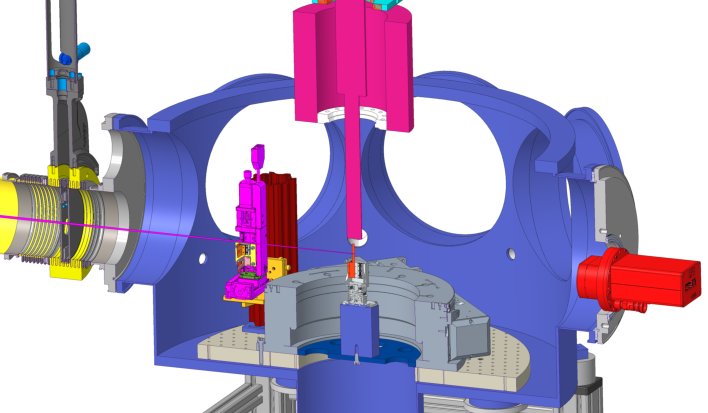
\includegraphics{images/aufbau/aufbau_empty.pdf}
    \caption{Die Skizze des Anlageaufbaus. Die Einzelbauteile sind farbig kodiert. In der Vakuumkammer (blau) wird der Druck in Höhe von ca. \SI{2.4e6}{\milli\bar} aufrechterhaltet. Der Probehalter (pink) ist aus Kupfer gemacht und kann die Rolle eines Wärmeleiters für die Probenkühlung spielen. Dazu ist der Probehalter mit der Kryoanlage angeschlossen. Der Probehalter lässt sich in. Der horizontale Spalt (fuchsia) dient zum Abschneiden des gewünschten Stahlsanduhrbereichs. Die Spaltlage sowie die Spaltbreite kann beliebig verstellt werden. Der MÖNCH-Detektor (rot) ist an der zum Strahlgang (gelb) gegenüberliegenden Wand der Vakuumkammer befestigt.}
    \label{fig:anlage}
\end{figure}
% Gd M4 = 1212eV 

\noindent
Die zu untersuchende mehrschichtige Probe (s. Abschnitt \ref{text:streuung}), wie bereits erwähnt wurde, besteht aus Gd und Fe. Mithilfe der \gls{rzp} wird die Energie der M5 Gd-Absorptionskante $E_{Gd, M5} = \SI{1185(1)}{\eV}$ \cite[Abb. 6(a)]{prieto_x-ray_2005} auf die Probe abgebildet.